\documentclass{standalone}
\usepackage{tikz}
\usetikzlibrary{arrows.meta, decorations.pathmorphing}

\begin{document}
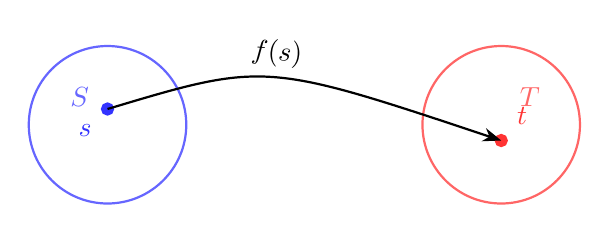
\begin{tikzpicture}[>=Stealth, thick]

  % Draw sets S and T as smaller circles
  \draw[blue!60, thick] (-2,0) circle (1.0cm) node[above left=3pt] {$S$};
  \draw[red!60, thick]  (3,0) circle (1.0cm) node[above right=3pt] {$T$};

  % Elements s and t (shifted slightly for better spacing)
  \filldraw[blue!80] (-2,0.2) circle (2pt) node[below left=2pt] {$s$};
  \filldraw[red!80]  (3,-0.2) circle (2pt) node[above right=2pt] {$t$};

  % Curved function arrow
  \draw[->, thick] 
    (-2,0.2) .. controls (0,0.8) .. (3,-0.2)
    node[midway, above, sloped] {$f(s)$};

\end{tikzpicture}
\end{document}
